\renewcommand{\FileName}{part3}

\part{n-way tables}
\begin{frame}
  \frametitle{Part 3: Mosaic displays and \loglin\ models}
 \begin{minipage}[c]{.33\textwidth}
  \includegraphics[width=1\linewidth]{fig/mosaic9a3f}
  \end{minipage}%
 \hfill
 \begin{minipage}[c]{.33\textwidth}
  \includegraphics[width=1\linewidth,clip]{fig/mosaic9a4f}
 \end{minipage}
 \hfill
 \begin{minipage}[c]{.33\textwidth}
  \includegraphics[width=1\linewidth,clip]{fig/mosmat9m}
 \end{minipage}

Topics:
  \begin{itemize*}
	\item Mosaic displays 
	\item \loglin\ models for \nway\ tables
%	\item Correspondence analysis
    \item Visualizing \loglin\ models: \proglang{SAS} \& \proglang{R}
    \item Models for square and structured tables
	\item Larger tables
  \end{itemize*}
\end{frame}

\section{n-way tables}
\renewcommand{\FileName}{mosbasic}

\subsection{Mosaic displays: Basic ideas}
\begin{frame}
  \frametitle{Mosaic displays: Basic ideas}
\citet{HartiganKleiner:81,Friendly:94a,Friendly:99b}
 \begin{columns}
   \begin{column}{.5\textwidth}
     \begin{itemize}
      \item Area-proportional display of frequencies in an $n$-way table
	  \item Tiles (cells): recursive splits of a unit square---
		\begin{itemize*}
		 \item<1-> V1: \alert{width} $\sim$ marginal frequencies, $n_{i++}$
		 \item<2-> V2: \alert{height} $\sim$ relative frequencies \given V1, $n_{ij+} / n_{i++}$
		 \item<3-> V3: \alert{width} $\sim$ relative frequencies \given (V1, V2), $n_{ijk} / n_{ij+}$
         \item<3-> $\cdots$
		\end{itemize*}
       \item $\Rightarrow$  area $\sim$ cell frequency, $n_{ijk}$
     \end{itemize}
   \end{column}
   \begin{column}{.5\textwidth}
      \includegraphics<1>[width=\linewidth]{fig/ucb0}
      \includegraphics<2>[width=\linewidth]{fig/ucb1}
      \includegraphics<3>[width=\linewidth]{fig/ucb4}
   \end{column}
 \end{columns}
\end{frame}


\begin{frame}
  \frametitle{Mosaic displays: Basic ideas}
 \begin{columns}
   \begin{column}{.5\textwidth}
     \begin{itemize}
      \item Independence: Two-way table
	  \item Expected frequencies: 
		\begin{equation*}
		 \widehat{m}_{ij} = \frac{n_{i+} n_{+j}}{n_{++}} = n_{++} \text{row \%} \text{col \%}
		\end{equation*}
       \item $\Rightarrow$  rows \& columns align when variables are independent
     \end{itemize}
   \end{column}
   \begin{column}{.5\textwidth}
      \includegraphics[width=\linewidth]{fig/ucb1e}
   \end{column}
 \end{columns}
\end{frame}

\begin{frame}
  \frametitle{Mosaic displays: Residuals \& shading}
 \begin{columns}
   \begin{column}{.5\textwidth}
     \begin{itemize}
%      \item Independence: Two-way table
	  \item \alert{Pearson residuals}: 
		\begin{equation*}
		 d_{ij} = \frac{n_{ij} - \widehat{m}_{ij} }{\sqrt{\widehat{m}_{ij}}}
		\end{equation*}
       \item Pearson $\chi^2 = \Sigma \Sigma d_{ij}^2 =  \Sigma \Sigma \frac{(n_{ij} - \hat{m}_{ij})^2}{\hat{m}_{ij}}$
       \item Other residuals: deviance (LR), Freeman-Tukey (FT), adjusted (ADJ), ...
       \item \alert{Shading}:
			\begin{itemize*}
			\item Sign: \red{$-$ negative in red}; \blue{$+$ positive in blue}
			\item Magnitude: intensity of shading:  $|d_{ij}| > 0, 2, 4, \dots$
			\end{itemize*}
       \item $\Rightarrow$ Independence:  rows align, or \alert{cells are empty}!
     \end{itemize}
   \end{column}
   \begin{column}{.5\textwidth}
      \includegraphics[width=\linewidth]{fig/ucb2}
   \end{column}
 \end{columns}
\end{frame}

\endinput

\subsection{Loglinear models: Overview}
\renewcommand{\FileName}{loglin}
% slide template
% slide template
\begin{frame}
  \frametitle{\Loglin\  models: Overview}
  \begin{block}{\large\bfseries Modeling perspectives}
      \begin{itemize}[<+->]
	    \item \alert{\Loglin} models can be developed as an analog of classical ANOVA and regression
		models, where \emph{multiplicative} relations (under independence) are re-expressed in \emph{additive}
		form as models for log(frequency).
          \begin{equation*}
          	 	\log m_{ij} = \mu + \lambda_i^A + \lambda_j^B 	\equiv [A] [B] \equiv \sim A + B
          \end{equation*}

		\item More generally, \loglin\ models are also \alert{generalized linear models}
        (GLMs) 
		for log(frequency), with a Poisson distribution for the cell counts.
			\[ \log \vec{m} = \mat{X}  \vec{\beta}\]

		\item When one table variable is a response, a \alert{logit model} for that response is equivalent
		to a \loglin\ model (discussed in Part 4).
          \begin{equation*}
          	 	\log (m_{1jk}/m_{2jk}) = \alpha + \beta_j^B + \beta_k^C	\equiv [AB] [AC] [BC]
          \end{equation*}
      \end{itemize}
  \end{block}
\end{frame}
	
\begin{frame}[allowframebreaks]
  \frametitle{\Loglin\  models: Overview}
  \begin{itemize}
   \item {\large\bfseries Two-way tables: \Loglin\ approach}
%      \begin{itemize*}

      For two discrete variables, $A$ and $B$, suppose a multinomial sample of total size $n$
	  over the $IJ$ cells of a two-way $I \times J$ contingency table, with cell frequencies
	  $n_{ij}$, and cell probabilities $\pi_{ij} = n_{ij}/n$.
    	\begin{itemize*}
	  	\item The table variables are \alert{statistically independent} when the cell (joint) probability equals
	  	the product of the marginal probabilities, $\Pr(A=i \:\&\: B=j) = \Pr(A=i) \times  \Pr(B=j)$, or,
	  	\[ \pi_{ij} = \pi_{i+} \pi_{+j} \period \]
	  	\item An equivalent model in terms of expected frequencies, $m_{ij} = n \pi_{ij}$ is
	  	\[ m_{ij} = (1/n) \: m_{i+} \: m_{+j} \period \]
%\framebreak
		\item This multiplicative model can be expressed in additive form as a model for $\log m_{ij}$,
	\begin{equation}\label{eq:logmij}
	 \log m_{ij} = -\log n + \log m_{i+} + \log m_{+j} \period
	\end{equation}
\framebreak
		\item By anology with ANOVA models, the independence model \eqref{eq:logmij} can be expressed as 
		\begin{equation}\label{eq:independence}
	 	\log m_{ij} = \mu + \lambda_i^A + \lambda_j^B \comma	
		\end{equation}
		where $\mu$ is the grand mean of $\log m_{ij}$ and the parameters $\lambda_i^A$ and  $\lambda_j^B$
		express the marginal frequencies of variables $A$ and $B$, and are typically defined so that
		 $\sum_i \lambda_i^A = \sum_j \lambda_j^B =0$.
		\end{itemize*}

	   Dependence between the table variables is expressed by adding association parameters,
		$\lambda_{ij}^{AB}$, giving the \emph{saturated model},
	\begin{equation}\label{eq:saturated}
	 	\log m_{ij} = \mu + \lambda_i^A + \lambda_j^B + \lambda_{ij}^{AB} \equiv [AB] \equiv \sim
		A*B \period  
	\end{equation}
		\begin{itemize*}
			\item The saturated model fits the table perfectly ($\widehat{m}_{ij} = n_{ij}$): 
			there are as many parameters as cell
			frequencies. Residual df = 0.
			\item A global test for association tests $H_0: \mat{\lambda}_{ij}^{AB} = \mat{0}$.
			\item For ordinal variables, the $\lambda_{ij}^{AB}$ may be structured more simply,
			giving tests for ordinal association.
		\end{itemize*}
%	  \end{itemize*}
  \end{itemize}
	
\end{frame}
%\framebreak
\begin{frame}	
  \begin{itemize}
	\item{\large\bfseries \large\bfseries Two-way tables: GLM approach}
		\begin{itemize}
			\item In the GLM approach, the vector of cell frequencies, $\vec{n} = \{ n_{ij}\}$ is specified
			to have a \alert{Poisson} distribution with means $\mat{m} = \{m_{ij}\}$ given by
			\[ \log \vec{m} = \mat{X}  \vec{\beta}\]
			where $\mat{X}$ is a known design (model) matrix and $\vec{\beta}$ is a column vector
			containing the unknown $\lambda$ parameters.
			\item For example, for
a $2\times 2$ table, the saturated model \eqref{eq:saturated} with the usual zero-sum constraints
can be represented as
\begin{equation*}
\left(
\begin{array}{c}
\log m_{11} \\
\log m_{12} \\
\log m_{21} \\
\log m_{22}
\end{array}
\right) =\left[
\begin{array}{rrrr}
1 & 1 & 1 & 1 \\
1 & 1 & -1 & -1 \\
1 & -1 & 1 & -1 \\
1 & -1 & -1 & 1
\end{array}
\right] \left(
\begin{array}{c}
\mu  \\
\lambda _1^A \\
\lambda _1^B \\
\lambda _{11}^{AB}
\end{array}
\right)
\end{equation*}
Note that only the linearly independent parameters are represented.
$\lambda_2^A = - \lambda_1^A$, because $\lambda_1^A + \lambda_2^A =0$, 
and so forth.
		\item Advantages of the GLM formulation: easier
to express models with ordinal or quantitative variables, special terms, etc. 
Can also allow for \emph{over-dispersion}. 
		\end{itemize} 
%	\item{\large\bfseries }
  \end{itemize}
\end{frame}

% slide template
\begin{frame}[allowframebreaks]
  \frametitle{Three-way Tables}
  \begin{itemize}
	\item{\large\bfseries Saturated model:} For a 3-way table, of size $I \times J \times K$ for variables $A, B, C$,
	 the saturated \loglin\ model includes associations between
	all pairs of variables, as well as a 3-way association term, $\lambda_{ijk}^{ABC}$
\begin{equation} \label{eq:lsat3}
  \begin{split}
  \log \,  m_{ijk}  
 = \mu  
& +  \lambda_i^A
  +  \lambda_j^B
  +  \lambda_k^C       \\
& +  \lambda_{ij}^{AB}
  +  \lambda_{ik}^{AC}
  +  \lambda_{jk}^{BC}
  +  \lambda_{ijk}^{ABC}
  \period
  \end{split}
\end{equation}
      \begin{itemize*}
	  \item One-way terms ($\lambda_i^A, \lambda_j^B, \lambda_k^C$):
	  differences in the \emph{marginal frequencies} of the table variables.
	  \item Two-way terms ($\lambda_{ij}^{AB}, \lambda_{ik}^{AC},\lambda_{jk}^{BC}$)
	  pertain to the \emph{partial association} for each pair of variables, \emph{controlling}
	  for the remaining variable.
	  \item The three-way term, $\lambda_{ijk}^{ABC}$ allows the partial association between any
	  pair of variables to vary over the categories of the third variable.
	  \item Such models are usually \emph{hierarchical}:  the presence of a high-order term, such as
	  $\lambda_{ijk}^{ABC}$ $\rightarrow$  \emph{all} low-order relatives are automatically included.
	  \item Thus, a short-hand notation for a \loglin\ model lists only the high-order terms,
	  i.e., model \eqref{eq:lsat3} $\equiv [ABC]$
%    	\begin{itemize*}
%		\item 
%		\item 
%		\end{itemize*}
	  \end{itemize*}
%\end{frame}
\framebreak
%\begin{frame}	
	\item{\large\bfseries Reduced models:}  

    The usual goal is to fit the \emph{smallest} model
	(fewest high-order terms) that is sufficient to explain/describe the observed frequencies.
%    	\begin{itemize*}
%		\item All representative subset models are shown in the table below
		\input{tab/loglin-3waya}
		Symbolic notation (high-order terms):
		\[  [AB][C] \equiv 
  \log \,  m_{ijk}  =
  \mu  +  \lambda_i^A +  \lambda_j^B  +  \lambda_k^C
  +  \lambda_{ij}^{AB}
		\] 
		\[  [AB][AC] \equiv 
  \log \,  m_{ijk}  =
  \mu  +  \lambda_i^A +  \lambda_j^B  +  \lambda_k^C
  +  \lambda_{ij}^{AB}
  +  \lambda_{ik}^{AC}
		\] 
%		\end{itemize*}

%\end{frame}
\framebreak
%\begin{frame}	
	\item{\large\bfseries Assessing goodness of fit}
    	\begin{itemize}
		\item Goodness of fit of a specified model may be tested by the likelihood ratio $G^2$,
\begin{equation}\label{eq:pgsq}
\GSQ =  2 \sum_i n_i \, \log ( n_i / \widehat{m}_i )
\comma
\end{equation}
		or the Pearson $\chisq$,
\begin{equation}\label{eq:pchi}
\chisq = \sum_i \frac{( n_i - \widehat{m}_i )^2}{\widehat{m}_i}
\comma
\end{equation}
	with degrees of freedom = \# cells - \#  estimated parameters.  
	\item E.g., for the model
	of mutual independence, $[A] [B] [C]$, df = $IJK - (I-1) - (J-1) - (K-1) = (I-1)(J-1)(K-1)$
	\item The terms summed in \eqref{eq:pgsq} and \eqref{eq:pchi} are the squared \emph{cell residuals}
	\item Other measures of balance goodness of fit against parsimony, e.g., \emph{Akaike's Information Criterion}
	(smaller is better)
	\[ AIC = \GSQ - 2 df \mbox{ or }  AIC = \GSQ + 2 \mbox{ \# parameters} \]
		\end{itemize}
  \end{itemize}
\end{frame}

\endinput

% slide template
\begin{frame}
  \frametitle{}
  \begin{itemize}
	\item{\large\bfseries }
      \begin{itemize*}
	  \item 
    	\begin{itemize*}
		\item 
		\item 
		\end{itemize*}
	  \item 
	  \end{itemize*}
	\item{\large\bfseries }
	\item{\large\bfseries }
  \end{itemize}
\end{frame}


\subsection{Loglinear models: Fitting}
\renewcommand{\FileName}{loglfit}
\begin{frame}[fragile]
 \frametitle{Fitting \loglin\ models: SAS}
 \begin{block}{SAS}
  \begin{itemize}
   \item \PROC{CATMOD}
\begin{Input}[baselinestretch=0.8,fontsize=\footnotesize]
%include catdata(berkeley);
proc catmod order=data data=berkeley;
   format dept dept. admit admit.;
   \sasemph{weight freq;}                  \sascomment{/* data in freq. form */}
   model dept*gender*admit=_response_ ;
   \sasemph{loglin} admit|dept|gender @2   / title='Model (AD,AG,DG)'; run;
   \sasemph{loglin} admit|dept dept|gender / title='Model (AD,DG)';  run;
\end{Input}

   \item \PROC{GENMOD}
\begin{Input}[baselinestretch=0.8,fontsize=\footnotesize]
proc genmod data=berkeley;
   class dept gender admit;
   model freq = dept|gender dept|admit / \sasemph{dist=poisson};
run;
\end{Input}

  \end{itemize}
 \end{block}
\begin{itemize*}
  \item \texttt{mosaic} macro usually fits loglin models internally and
  displays results
  \item You can also use \PROC{GENMOD} for a more general model, and
  display the result with the \texttt{mosaic} macro.
\end{itemize*}
  
\end{frame}

\begin{frame}[fragile]
 \frametitle{Fitting \loglin\ models: R}
 \begin{block}{R}
  \begin{itemize}
   \item \func{loglm} - data in contingency table form (\pkg{MASS})
\begin{Input}[baselinestretch=0.8,fontsize=\footnotesize]
data(UCBAdmissions)
  ## conditional independence (AD, DG) in Berkeley data
mod.1 <- loglm(~ (Admit + Gender) * Dept, data=UCBAdmissions)
  ## all two-way model (AD, DG, AG) 
mod.2 <- loglm(~ (Admit + Gender + Dept)^2, data=UCBAdmissions)
\end{Input}

   \item \func{glm} - data in frequency form
\begin{Input}[baselinestretch=0.8,fontsize=\footnotesize]
berkeley <- as.data.frame(UCBAdmissions)
mod.3 <- glm(Freq ~ (Admit + Gender) * Dept, data=berkeley, 
                   \sasemph{family='poisson'})
\end{Input}

  \end{itemize}
 \end{block}

\begin{itemize*}
  \item \func{loglm} simpler for nominal variables
  \item \func{glm} allows a wider class of models
  \item \func{gnm} fits models for structured association and
  generalized \emph{non-linear} models
  \item \texttt{vcdExtra} package provides visualizations for all.
  
\end{itemize*}

\end{frame}


\subsection{Mosaic displays}
\renewcommand{\FileName}{nway2}

% these two frames covered in mosbasic
\begin{comment}
\begin{frame}
%\makeatletter\slidebox@restore\makeatother
\frametitle{Mosaic displays and Log-linear Models}
\citet{HartiganKleiner:81,Friendly:94a,Friendly:99b}:
\begin{itemize}
\item \boldital{Width} $\sim$ one set of marginals, $n_{i+}$
\item \boldital{Height} $\sim$ relative proportions of other variable, 
$p_{j\given i} = n_{ij} / n_{i+}$
\item $\Rightarrow$ \textbf{area} $\sim$ \textbf{frequency}, $n_{ij} = n_{i+} p_{j\given i}$
\begin{center}
  \includegraphics[width=.5\dispwidth,clip]{fig/mosaic9a1f}
\end{center}
\end{itemize}
\end{frame}

\begin{frame}
\begin{itemize}
\item \boldital{Shading}: Sign and magnitude of Pearson
$\chi^2$ residual,
$d_{ij} = ( n_{ij} - \hat{m}_{ij} ) / \sqrt{\hat{m}_{ij}}$ (or L.R. $G^2$)
\begin{itemize*}
\item Sign: \red{$-$ negative in red}; \blue{$+$ positive in blue}\black
\item Magnitude: intensity of shading:  $|d_{ij}| > 0, 2, 4, \dots$
\end{itemize*}
\item \boldital{Independence}: Rows $\approx$ align, \emph{or}
cells are empty!
\item E.g., aggregate Berkeley data, independence model:
\end{itemize}

\begin{center}
  \includegraphics[width=.5\dispwidth,clip]{fig/mosaic9a1f}
\end{center}
\end{frame}
\end{comment}

\begin{frame}
  \frametitle{Mosaic displays: Hair color and eye color}
  \vspace{2ex}
 \begin{minipage}[c]{.49\dispwidth}
  \includegraphics[width=1\linewidth,clip]{fig/mosaic3m1}
 \end{minipage}%
 \hfill
 \begin{minipage}[c]{.49\dispwidth}
  We know that hair color and eye color are associated ($\chi^2 (9) = 138.29$).
  The question is \alert{how}?
  \begin{itemize}
  \item Dark hair goes with dark eyes, light hair with light eyes
  \item Red hair, hazel eyes an exception?
  \item Effect ordering: Rows/cols permuted by CA Dimension 1
  \item[$\Rightarrow$] Opposite corner pattern
  \end{itemize}
 \end{minipage}
\end{frame}

\begin{frame}
\frametitle{Mosaic displays: Marginal models}
Berkeley data: Departments $\times$ Gender (ignoring Admit):
\begin{itemize}
\item Did departments differ in the total number of applicants?
\item Did men and women apply differentially to departments?
%\item Model [Dept] [Gender]: $G^2_{(5)} =$ 1220.6.
\end{itemize}

 \begin{minipage}[c]{.49\dispwidth}
  \includegraphics[width=1\linewidth,clip]{fig/mosaic9a2f}
 \end{minipage}%
 \hfill
 \begin{minipage}[c]{.49\dispwidth}
\begin{itemize*}
\item Model [Dept] [Gender]: $G^2_{(5)} =$ 1220.6.
\item \boldital{Note}: Departments ordered A--F by overall rate of admission.
\end{itemize*}
 \end{minipage}
	
\end{frame}

\begin{frame}
\frametitle{Mosaic displays for multiway tables}
\begin{itemize}
\item Generalizes to $n$-way tables: divide cells recursively
\item Can fit \emph{any} log-linear model (e.g., 2-way, 3-way, $\dots$),
	\begin{itemize*}
	\item For a 3-way table:  [A][B][C], [AB][C], [AB][AC], $\dots$, [ABC]
	\end{itemize*}

%\scalebox{.9}{%
%\input{tab/loglin-3way}
%}

%e.g., the model for conditional independence ($A \perp C \given B$):
%\begin{equation*}
%[AB][BC] \equiv
%  \log \,  m_{ijk}  =
%  \mu
%  +  \lambda_i^A
%  +  \lambda_j^B
%  +  \lambda_k^C
%  +  \lambda_{ij}^{AB}
%  +  \lambda_{jk}^{BC}
%\end{equation*}

\item Each mosaics shows:
	\begin{itemize*}
	\item  \alert{\textbf{DATA}} (size of tiles)
	\item (some) \alert{\textbf{marginal}} frequencies (spacing $\rightarrow$ visual grouping)
	\item  \alert{\textbf{RESIDUALS}} (shading) --- what associations have been omitted?
	\end{itemize*}
\item Visual fitting:
	\begin{itemize*}
	\item Pattern of lack-of-fit (residuals) $\rightarrow$ ``better'' model---
	smaller residuals 
	\item ``cleaning the mosaic'' $\rightarrow$ ``better'' model---
	empty cells
	\item best done interactively!
	\end{itemize*}
\end{itemize}

\end{frame}

\begin{frame}
\begin{itemize}
\item E.g., Joint independence, [DG][A] (null model, Admit as response)
[$G^2_{(11)}$ = 877.1]:
\end{itemize}
\begin{center}
  \includegraphics[width=.55\dispwidth,clip]{fig/mosaic9a3f}
\end{center}
\end{frame}

\begin{frame}
%\makeatletter\slidebox@restore\makeatother
%\iflandscape\def\dispfactor{.5}\else \def\dispfactor{.7}\fi
\frametitle{Mosaic displays for multiway tables}
\begin{itemize}
\item Visual fitting:
%	\begin{itemize*}
%	\item Pattern of lack-of-fit (residuals) $\rightarrow$ ``better'' model---
%	smaller residuals 
%	\item ``cleaning the mosaic'' $\rightarrow$ ``better'' model---
%	empty cells
%	\item best done interactively!
%	\end{itemize*}
\end{itemize}

 \begin{minipage}[c]{.55\dispwidth}
  \includegraphics[width=1\linewidth,clip]{fig/mosaic9a4f}
 \end{minipage}%
 \hfill
 \begin{minipage}[c]{.44\dispwidth}
  \begin{itemize}
  \item E.g., Add [Dept Admit] association $\rightarrow$ Conditional independence: 
   \begin{itemize*}
   \item Fits poorly: ($G^2_{(6)}$ = 21.74)
   \item But, only in Department A!
   \end{itemize*}
   \item The GLM approach allows fitting a special term for Dept. A
   \item Technical note:  These displays use \emph{standardized residuals}: better
    statistical properties. 
  \end{itemize}
 \end{minipage}
\end{frame}

\begin{frame}
  \frametitle{Other variations: Double decker plots}
	 \begin{itemize*}
		 \item Visualize dependence of one categorical (typically binary) variable on predictors
		 \item Formally: mosaic plots with vertical splits for all \alert{predictor dimensions}, highlighting the
		 response by shading
	 \end{itemize*}
 \begin{center}
%	\setkeys{Gin}{width=.75\textwidth}
\includegraphics[width=.75\textwidth]{fig/plt-UCB-doubledecker}
 \end{center}
\end{frame}


\subsection{Sequential plots and models}
\begin{frame}
  \frametitle{Sequential plots and models}
  \begin{itemize}
	\item Mosaic for an \nway\ table $\rightarrow$ hierarchical decomposition of association in a way
analogous to \alert{sequential fitting} in regression
    \item Joint cell probabilities are decomposed as
\begin{equation*}
p_{ijk\ell \cdots} = \underbrace{\overbrace{p_i \times p_{j|i}}^{\{v_1 v_2\}} \times \: p_{k|ij}}_{\{v_1 v_2 v_3\}}
       \times \: p_{\ell|ijk} \times\cdots \times p_{n|ijk\cdots}
\end{equation*}
	
      \begin{itemize*}
	  \item First 2 terms $\rightarrow$ mosaic for $v_1$ and $v_2$
	  \item First 3 terms $\rightarrow$ mosaic for $v_1$, $v_2$ and $v_3$
	  \item $\cdots$
	  \end{itemize*}
	\item Sequential models of \emph{joint independence} $\rightarrow$
	additive decomposition of the total association,
	$G^2_{[v_1] [v_2] \dots [v_p]}$ (mutual independence),
\begin{equation*}
G^2_{[v_1] [v_2] \dots [v_p]} =
G^2_{[v_1] [v_2]} +
G^2_{[v_1 v_2] [v_3]} +
G^2_{[v_1 v_2 v_3] [v_4]} + \cdots+
G^2_{[v_1 \dots v_{p-1}] [v_p]}
\end{equation*}
   \item As in regression, most useful when there is some \alert{substantive ordering} of the variables
 \end{itemize}

\end{frame}

\begin{frame}
   \frametitle{Sequential plots and models: Example}
%\iflandscape\def\dispfactor{.65}\else \def\dispfactor{.7}\fi
  \begin{itemize}
    \item Hair color x Eye color marginal table (ignoring Sex)
  \end{itemize}
\begin{center}
  \includegraphics[width=.6\dispwidth,clip]{fig/mosaic3mj2}
\end{center}
   
\end{frame}

\begin{frame}
   \frametitle{Sequential plots and models: Example}
  \begin{itemize}
    \item 3-way table, Joint Independence Model [Hair Eye] [Sex]
  \end{itemize}
\begin{center}
  \includegraphics[width=.6\dispwidth,clip]{fig/mosaic3mj3}
\end{center}
   
\end{frame}

\begin{frame}
   \frametitle{Sequential plots and models: Example}
  \begin{itemize}
    \item 3-way table, Mutual Independence Model [Hair] [Eye] [Sex]
  \end{itemize}
\begin{center}
  \includegraphics[width=.6\dispwidth,clip]{fig/mosaic3mj1}
\end{center}
   
\end{frame}

\begin{frame}
   \frametitle{Sequential plots and models: Example}
%% three subfig side-by-side
 \begin{minipage}[c]{.3\textwidth}
  \centering Marginal 
  \\ \includegraphics[width=1\linewidth,clip]{fig/mosaic3mj2}
  \\ \centering [Hair] [Eye]
  \\ \centering $G^2_{(9)} = 146.44$
 \end{minipage}%
 \hfill {\Large +} \hfill
 \begin{minipage}[c]{.3\textwidth}
  \centering Joint 
  \\ \includegraphics[width=1\linewidth,clip]{fig/mosaic3mj3}
  \\ \centering [Hair Eye] [Sex]
  \\ \centering $G^2_{(15)} = 19.86$
 \end{minipage}
 \hfill {\Large =} \hfill
 \begin{minipage}[c]{.3\textwidth}
  \centering Total 
  \\ \includegraphics[width=1\linewidth,clip]{fig/mosaic3mj1}
  \\ \centering [Hair] [Eye] [Sex]
  \\ \centering $G^2_{(24)} = 166.30$
 \end{minipage}
 
\end{frame}

% slide template
\subsection{Mosaic matrices}
\begin{frame}
  \frametitle{Mosaic matrices}
  \begin{itemize}
	\item Analog of \emph{scatterplot matrix} for categorical data \citep{Friendly:99b}
      \begin{itemize*}
	  \item Shows all $p (p-1)$ pairwise views in a coherent display
	  \item Each pairwise mosaic shows bivariate (marginal) relation
	  \item Fit: marginal independence
	  \item Residuals: show \alert{marginal} associations
	  \item Direct visualization of the ``Burt'' matrix analyzed in
	  MCA for $p$ categorical variables
	  \end{itemize*}
  \end{itemize}
\begin{center}
  \includegraphics[width=.4\dispwidth,clip]{fig/mosmat3}
\end{center}
\end{frame}

\begin{frame}
  Hair, Eye, Sex data:
\begin{center}
  \includegraphics[height=.94\textheight,clip]{fig/mosmat3}
\end{center}
\end{frame}

\begin{frame}
Berkeley data: %(does not display)
\begin{center}
  \includegraphics[height=.94\textheight,clip]{fig/mosmat9m}
\end{center}
\end{frame}

\subsection{Partial association}
\begin{frame}
  \frametitle{Partial association, Partial mosaics}
  \begin{itemize}
	\item{\large\bfseries Stratified analysis:}
      \begin{itemize*}
	  \item How does the association between two (or more) variables vary 
	  over levels of other variables?
	  \item Mosaic plots for the main variables show \emph{partial association}
	  at each level of the other variables.
%	  \item Analog of \emph{coplot} (conditioning plot) for categorical data
	  \item E.g., Hair color, Eye color \emph{BY} Sex $\leftrightarrow$ 
	  \texttt{TABLES sex * hair * eye;}
      \end{itemize*}
  \end{itemize}
\begin{center}
  \includegraphics[width=.86\dispwidth,clip]{fig/mospart3}
\end{center}

\end{frame}

\begin{frame}

  \frametitle{Partial association, Partial mosaics}
  \begin{block}{\large\bfseries Stratified analysis: conditional decomposition of $G^2$}
      \begin{itemize*}
	  \item Fit models of partial (conditional) independence, $ A \perp B \given C_k$
            at each level of (controlling for) $C$.
	  \item $\Rightarrow$ partial $G^2$s add to the overall
	  $G^2$ for conditional independence,$ A \perp B \given C$
\begin{equation*}
G^2_{A \perp B \given C} = \sum_k G^2_{A \perp B \given C(k)}
\end{equation*}
       \end{itemize*}
 \end{block}

\input{tab/haireyesex}
\end{frame}


%\input{frames/dummy}

\endinput

% two figures 
 \begin{minipage}[b]{.5\linewidth}
  \centering
  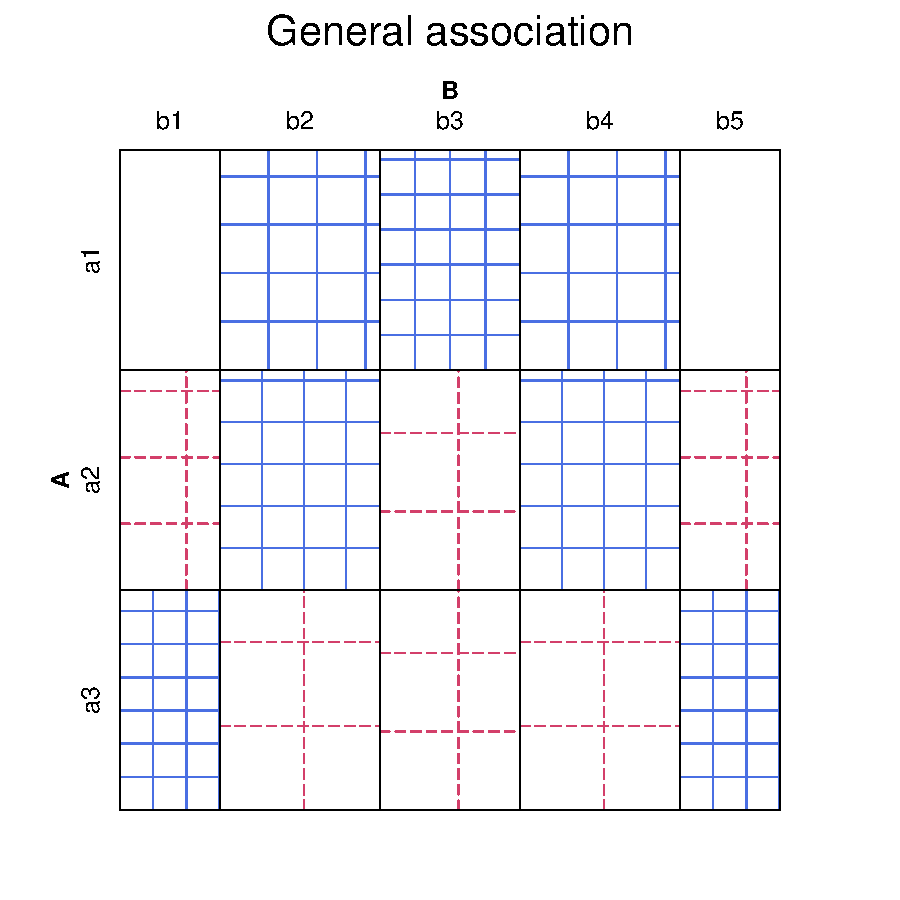
\includegraphics[width=.95\linewidth]{fig/cmhdemo1}
 \end{minipage}%
 \begin{minipage}[b]{.5\linewidth}
  \centering
  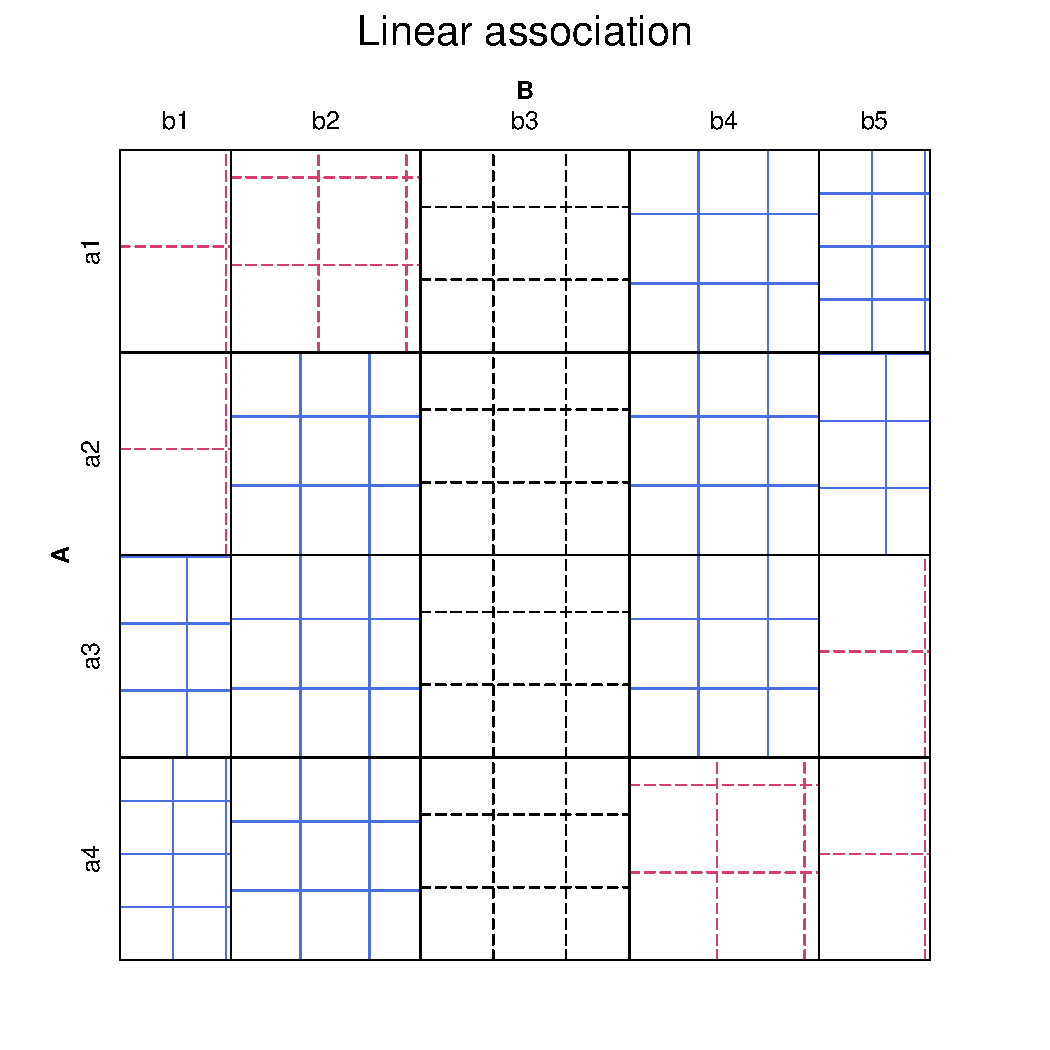
\includegraphics[width=.95\linewidth]{fig/cmhdemo2}
 \end{minipage}

% slide template
\begin{frame}
  \frametitle{}
  \begin{itemize}
	\item{\large\bfseries }
      \begin{itemize*}
	  \item 
    	\begin{itemize*}
		\item 
		\item 
		\end{itemize*}
	  \item 
	  \end{itemize*}
	\item{\large\bfseries }
	\item{\large\bfseries }
  \end{itemize}
\end{frame}



\section{Mosaics software}
%\input{frames/dummy}
%\begin{comment}	
\renewcommand{\FileName}{mossoft}

\subsection{Web applet}
\begin{frame}
  \frametitle{Software for Mosaic Displays: Web applet}
  \begin{block}{\large\bfseries Demonstration web applet}
	Go to: \url{http://datavis.ca/online/mosaics/}
	\begin{itemize}
		\item Runs the \emph{current} version of \texttt{mosaics.sas} via a cgi script (perl)
		\item Can:
		\begin{itemize*}
		  \item run \emph{sample} data, 
		  \item \emph{upload} a data file, 
		  \item \emph{enter} data in a form.
		\end{itemize*}
		\item Choose model \emph{fitting} and \emph{display} options (not all supported).
		\item Provides (limited) interaction with the mosaics via javascript
	\end{itemize}
  \end{block}
\end{frame}


\begin{frame}[plain]
\begin{center}
  \includegraphics[width=.9\dispwidth,clip]{fig/mosaic-cgi1a}
%  \includegraphics[width=.95\linewidth]{\vcdguide{mosaic-cgi}}
\end{center}
\end{frame}

\begin{frame}[plain]
\begin{center}
  \includegraphics[width=.9\dispwidth,clip]{fig/mosaic-cgi2a}
\end{center}
\end{frame}
%\end{comment}

\subsection{SAS}
\begin{frame}
  \frametitle{Software for Mosaic Displays: SAS}
  \begin{block}{\large\bfseries SAS software \& documentation}
	\url{http://datavis.ca/mosaics/mosaics.pdf} - User Guide
	\url{http://datavis.ca/books/vcd/macros.html} - Software

   \begin{itemize}
	\item {\large\bfseries Examples}: Many in \VCD{} and on web site

	\item{\large\bfseries \IML{} modules}: \texttt{mosaics.sas}--- Most flexible
      \begin{itemize*}
	  \item Enter frequency table directly in \IML{}, or read from a SAS \Dset{}.
%	  \item Most flexible:
%    	\begin{itemize*}
		\item Select, collapse, reorder, re-label table levels using \IML{} statements
		\item Specify structural 0s, fit specialized models (e.g., quasi-independence)
		\item Interface to models fit using \PROC{GENMOD}
%		\end{itemize*}
      \end{itemize*}
    \end{itemize}
  \end{block}

\end{frame}

\begin{frame}
  \frametitle{Software for Mosaic Displays: SAS}

  \begin{itemize}
	\item{\large\bfseries Macro interface}: \macro{mosaic}, \macro{table}, \macro{mosmat}
	\item{\large\bfseries \macro{mosaic}}--- Easiest to use
%      \begin{itemize*}
%	  \item Easiest to use:
    	\begin{itemize*}
		\item Direct input from a SAS \Dset{}
		\item No knowledge of \IML{} required
		\item Reorder table variables; collapse, reorder table levels with \macro{table}
		\item Convenient interface to \emph{partial mosaics} (\texttt{BY=})
		\end{itemize*}
%	  \end{itemize*}

	\item{\large\bfseries \macro{table}}
      \begin{itemize*}
	  \item Create frequency table from raw data
	  \item Collapse, reorder table categories
	  \item Re-code table categories using SAS formats, e.g., \texttt{1='Male' 2='Female'}
	  \end{itemize*}
	\item{\large\bfseries \macro{mosmat}}
      \begin{itemize*}
	  \item Mosaic matrices--- analog of scatterplot matrix \citep{Friendly:99b}
	  \end{itemize*}
  \end{itemize}
\end{frame}

% slide template
\begin{frame}[fragile]
  \frametitle{\macrot{mosaic} example: Berkeley data}
\begin{Input}[fontsize=\small,label=\fbox{\texttt{berkeley.sas}},baselinestretch=0.7]
title 'Berkeley Admissions data';
proc format;
   value admit 1="Admitted" 0="Rejected"          ;
   value dept  1="A" 2="B" 3="C" 4="D" 5="E" 6="F";
        value $sex  'M'='Male'   'F'='Female';\ignore{$}
data berkeley;
   do dept = 1 to 6;
      do gender = 'M', 'F';
         do admit = 1, 0;
            input freq @@;
            output;
   end; end; end;
\sascomment{/* -- Male --  - Female- */}
\sascomment{/* Admit  Rej  Admit Rej */}
datalines;
     512  313    89   19  \sascomment{/* Dept A */}
     353  207    17    8  \sascomment{/*      B */}
     120  205   202  391  \sascomment{/*      C */}
     138  279   131  244  \sascomment{/*      D */}
      53  138    94  299  \sascomment{/*      E */}
      22  351    24  317  \sascomment{/*      F */}
;
\end{Input}
\end{frame}

\begin{frame}[fragile]
Data set \texttt{berkeley}:
\begin{Output}[gobble=9,baselinestretch=0.7]
                  dept    gender    admit    freq

                    1       M         1       512
                    1       M         0       313
                    1       F         1        89
                    1       F         0        19
                    2       M         1       353
                    2       M         0       207
                    2       F         1        17
                    2       F         0         8
                    3       M         1       120
                    3       M         0       205
                    3       F         1       202
                    3       F         0       391
                    4       M         1       138
                    4       M         0       279
                    4       F         1       131
                    4       F         0       244
                    5       M         1        53
                    5       M         0       138
                    5       F         1        94
                    5       F         0       299
                    6       M         1        22
                    6       M         0       351
                    6       F         1        24
                    6       F         0       317
\end{Output}

\end{frame}

\begin{frame}[fragile]
  \frametitle{\macrot{mosaic} example: Berkeley data}
\begin{Input}[fontsize=\small,label=\fbox{\texttt{mosaic9m.sas}},baselinestretch=0.9]
goptions hsize=7in vsize=7in;
%include catdata(berkeley);
 
\sascomment{*-- apply character formats to numeric table variables;}
%table(data=berkeley, 
    var=Admit Gender Dept,
    weight=freq,
    char=Y, format=admit admit. gender $sex. dept dept.,\ignore{$}
    order=data, out=berkeley);
 
%mosaic(data=berkeley, 
    vorder=Dept Gender Admit, \sascomment{/* reorder variables */}
    plots=2:3,                \sascomment{/* which plots?      */}
    fittype=joint,            \sascomment{/* fit joint indep.  */} 
    split=H V V, htext=3);    \sascomment{/* options           */}
\end{Input}
NB: 
The \texttt{fittype=} argument allows various types of sequential models: joint, conditional, etc.

\end{frame}

\begin{frame}
  \frametitle{\macrot{mosaic} example: Berkeley data}
%% two subfig side-by-side
 \begin{minipage}[t]{.45\textwidth}
  \includegraphics[width=1\linewidth,clip]{fig/mosaic9a2f}
  \\ \centering Two-way, Dept. by Gender
 \end{minipage}%
 \hfill
 \begin{minipage}[t]{.45\textwidth}
  \includegraphics[width=1\linewidth,clip]{fig/mosaic9a3f}
  \\ \centering Three-way, Dept. by Gender by Admit
 \end{minipage}

 
\end{frame}

%\begin{fullversion}
\begin{comment}
\begin{frame}[fragile]
  \frametitle{\IML\ example}
\begin{Verbatim}[fontsize=\small,label=\fbox{\texttt{mosaic9.sas}},baselinestretch=0.7]
proc iml;
   \sascomment{*-- Berkeley Admissions data;}
   dim = \{2 2 6\};
   vnames = \{"Admit" "Gender" "Dept"\};       \sascomment{/* var names   */}
   lnames = \{                                \sascomment{/* level names */}
     "Admitted" "Rejected" " "  " "  " "  " ",
     "Male"  "Female" " "  " "  " "  " ",
     "A" "B" "C" "D" "E" "F"\};
          \sascomment{/* Admit Not Admit Not */}
   table = \{ 512  313,   89   19,
             353  207,   17    8,
             120  205,  202  391,
             138  279,  131  244,
              53  138,   94  299,
              22  351,   24  317\};
   reset storage=mosaic.mosaic;
   \sasemph{load module=_all_;}          \sascomment{*-- Load mosaic modules;}

   title = 'Model: &MODEL';
   plots=2:3;
   fittype='joint';
   \sasemph{run mosaic(dim, table, vnames, lnames, plots, title);}
 quit;
\end{Verbatim}
\end{frame}
\end{comment}
%\end{fullversion}

\begin{frame}[fragile]
  \frametitle{\macrot{mosmat}: Mosaic matrices}
  \vspace{1.5ex}

\begin{Input}[label=\fbox{\texttt{mosmat9m.sas}}]
%include catdata(berkeley);
%mosmat(data=berkeley, 
   vorder=Admit Gender Dept, sort=no);
\end{Input}
	  \vspace{.5ex}
	  \begin{center}
	  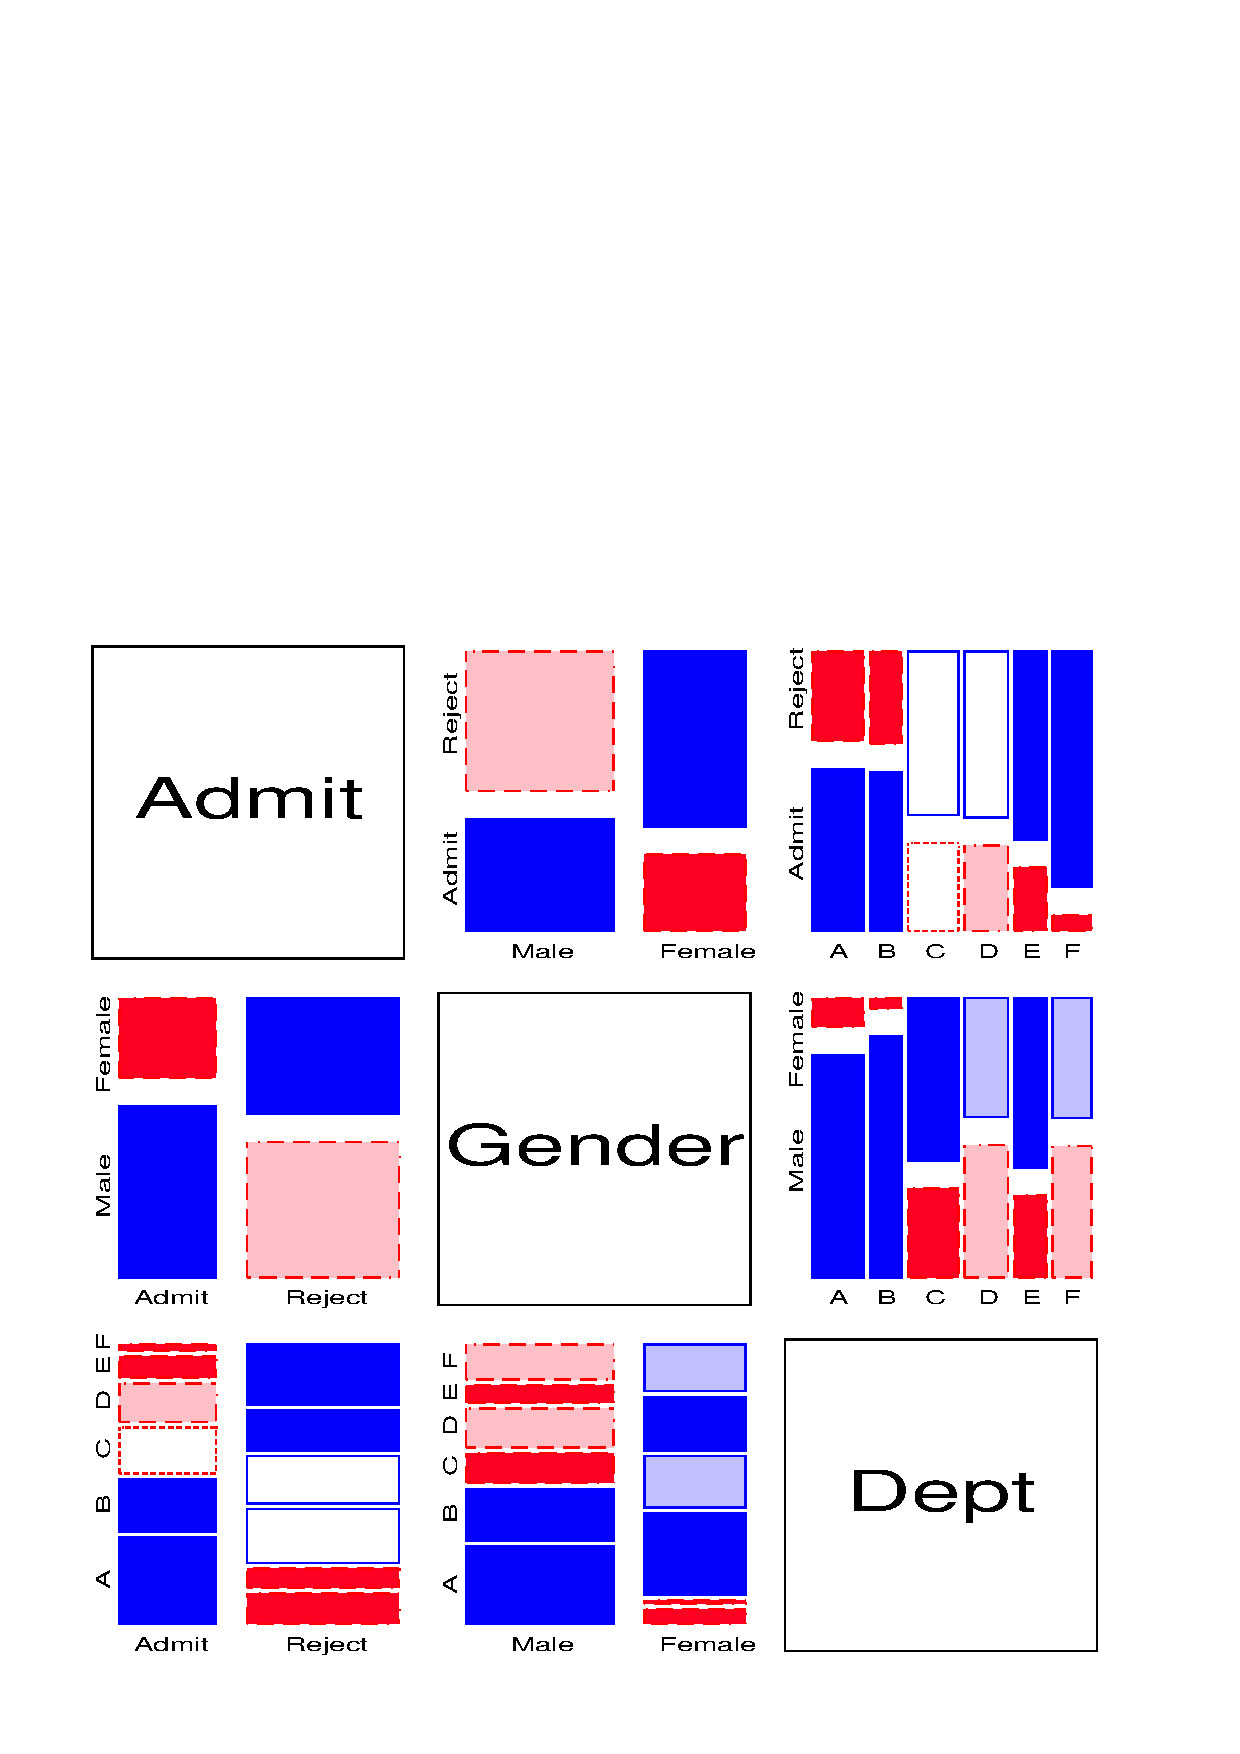
\includegraphics[width=.48\textwidth,clip]{fig/mosmat9a}
	  \end{center}
\end{frame}

\begin{frame}[fragile]
  \frametitle{Partial mosaics}
	  \vspace{1ex}

\begin{Input}[label=\fbox{\texttt{mospart3.sas}},baselinestretch=0.8,fontsize=\footnotesize]
%include catdata(hairdat3s);
%gdispla(OFF);
%mosaic(data=haireye, 
    vorder=Hair Eye Sex, \sasemph{by=Sex}, 
    htext=2, cellfill=dev);
%gdispla(ON);
%panels(rows=1, cols=2);     \sascomment{/* make 2 figs -> 1 */}
\end{Input}

\begin{center}
  \includegraphics[width=.85\dispwidth,clip]{fig/mospart3}
\end{center}
\end{frame}


\subsection{vcd package in R}
\renewcommand{\FileName}{R-ex1}
% slide template
\begin{frame}[fragile]
  \frametitle{Using the \texttt{vcd} package in R}
\begin{Rin}
>library(vcd)         # load the vcd package & friends
>
>data(HairEyeColor)
>structable(Eye ~ Hair + Sex, data=HairEyeColor)
\end{Rin}
\begin{Rout}[baselinestretch=0.85]
             Eye Brown Blue Hazel Green
Hair  Sex                              
Black Male          32   11    10     3
      Female        36    9     5     2
Brown Male          53   50    25    15
      Female        66   34    29    14
Red   Male          10   10     7     7
      Female        16    7     7     7
Blond Male           3   30     5     8
      Female         4   64     5     8
\end{Rout}
\begin{itemize*}
 \item The \func{structable} function $\rightarrow$`flat' representation of an $n$-way table, similar to mosaic displays
 \item Formula interface:  Col factors $\sim$ row factors
\end{itemize*}
% \begin{Rin}
% R>structable(Eye ~ Hair + Sex, data=HairEyeColor)
% \end{Rin}

\end{frame}

\begin{frame}[fragile]
  \frametitle{Using the \texttt{vcd} package in R}
\begin{itemize*}
  \item The \func{loglm} function fits a \loglin\ model, 
  returns a \texttt{loglm} object
   \begin{itemize*}
     \item Fit the 3-way mutual independence model: \texttt{Hair + Eye + Sex} $\equiv$ [Hair] [Eye] [Sex]
     \item Printing the object gives a brief model summary (badness of fit)
   \end{itemize*}
\begin{Rin}
>## Independence model of hair and eye color and sex.  
>mod.1 <- loglm(~Hair+Eye+Sex, data=HairEyeColor)
>mod.1
\end{Rin}
\begin{Rout}
Call:
loglm(formula = ~Hair + Eye + Sex, data = HairEyeColor)

Statistics:
                      X^2 df P(> X^2)
Likelihood Ratio 166.3001 24        0
Pearson          164.9247 24        0
\end{Rout}
  \item The \func{mosaic} function plots the object.
  \item the \texttt{vcdExtra} package extends \func{mosaic} to \func{glm}
  models.
\end{itemize*}

\end{frame}

\begin{frame}[fragile]
\begin{Rin}
>mosaic(mod.1, main="model: [Hair][Eye][Sex]")
\end{Rin}
 \begin{center}
 \includegraphics[width=.65\textwidth,clip]{R/haireyesex1}
 \end{center}

\end{frame}

\begin{frame}[fragile]

\frametitle{\pkg{vcd}: Other models}

\begin{Rin}
>## Joint independence model.  
>mod.2 <- loglm(~Hair*Eye+Sex, data=HairEyeColor)
>mod.2
\end{Rin}
\begin{Rout}[baselinestretch=0.9]
Call:
loglm(formula = ~Hair * Eye + Sex, data = HairEyeColor)

Statistics:
                      X^2 df  P(> X^2)
Likelihood Ratio 19.85656 15 0.1775045
Pearson          19.56712 15 0.1891745
\end{Rout}
\begin{Rin}
>## Conditional independence model:  Hair*Eye + Sex*Eye
>mod.3 <- loglm(~(Hair+Sex)*Eye, data=HairEyeColor)
>mod.3
\end{Rin}
\begin{Rout}[baselinestretch=0.9]
Call:
loglm(formula = ~(Hair + Sex) * Eye, data = HairEyeColor)

Statistics:
                      X^2 df  P(> X^2)
Likelihood Ratio 18.32715 12 0.1061122
Pearson          18.04110 12 0.1144483
\end{Rout}
\end{frame}

\begin{frame}[fragile]
\begin{Rin}
>mosaic(mod.2,  main="model: [HairEye][Sex]")
\end{Rin}
 \begin{center}
 \includegraphics[width=.65\textwidth,clip]{R/haireyesex2}
 \end{center}

\end{frame}

\begin{frame}[fragile]
\begin{Rin}
>mosaic(mod.2,  main="model: [HairEye][Sex]", gp=shading_Friendly)
R\end{Rin}
 \begin{center}
 \includegraphics[width=.65\textwidth,clip]{R/haireyesex2a}
 \end{center}

\end{frame}
\begin{frame}[fragile]
\frametitle{Testing differences between models}
\begin{itemize*}
  \item For \alert{nested models}, $M_1 \subset M_2$ ($M_1$ nested within, a special
  case of $M_2$), 
  the difference in LR $G^2$,
  $\Delta = G^2 (M_1) - G^2 (M_2)$
  is a \alert{specific test of the difference} between
  them.  Here, $\Delta \sim \chi^2$ with $df = df_1 - df_2$.
  \item R functions are object-oriented: they do different things for
  different types of objects.
\end{itemize*}

\begin{Rin}
>anova(mod.1, mod.2)
\end{Rin}
\begin{Rout}
LR tests for hierarchical log-linear models

Model 1:
 ~Hair + Eye + Sex 
Model 2:
 ~Hair * Eye + Sex 

           Deviance df Delta(Dev) Delta(df) P(> Delta(Dev)
Model 1   166.30014 24                                    
Model 2    19.85656 15  146.44358         9         0.0000
Saturated   0.00000  0   19.85656        15         0.1775
\end{Rout}

\end{frame}


\section{Structured tables}
\subsection{Ordinal variables}
\renewcommand{\FileName}{structured}
% slide template
\begin{frame}
  \frametitle{More structured tables}
  \begin{block}<1->{\large\bfseries Ordered categories}
      Tables with ordered categories may allow more \alert{parsimonious} tests of association
      \begin{itemize*}
	  \item Can represent $\lambda_{ij}^{AB}$ by a small number of parameters
	  \item $\rightarrow$ more focused and \emph{more powerful} tests of lack of independence (recall: CMH tests)
          \item Allow one to ``explain'' the \alert{pattern} of association in a compact way.
	  \end{itemize*}
  \end{block}

   \begin{block}<2->{\large\bfseries Square tables}
	For square $I \times I$ tables, where row and column variables have the
		same categories:
      \begin{itemize*}
	  	\item Can ignore diagonal cells, where association is expected and test
		remaining association (\emph{quasi-independence})
		\item Can  test whether association is \emph{symmetric} around the diagonal cells.
		\item Can test \alert{substantively important} hypotheses (e.g., mobility tables)
      \end{itemize*}
  \end{block}
  \uncover<2->{All of these require the GLM approach for model fitting}
\end{frame}

% slide template
\begin{frame}[allowframebreaks]
  \frametitle{Ordered categories}
  \begin{itemize}
	\item{\large\bfseries Ordinal scores}
      \begin{itemize*}
	  \item In many cases it may be reasonable to assign numeric scores, $\{a_i\}$
	  to an ordinal row variable and/or numeric scores, $\{b_i\}$ to an ordinal column variable.
	  \item Typically, scores are equally spaced and sum to zero, 
		$\{ a_i \} = i - (I+1)/2$, e.g., $\{ a_i \} = \{ -1, 0, 1 \}$ for I=3.
      \end{itemize*}
	  
	\item{\large\bfseries Linear-by-Linear (Uniform) Association}:
	  When \emph{both} variables are ordinal, the simplest model posits that any association
	  is \emph{linear} in both variables.
	  \[ \lambda_{ij}^{AB} = \gamma \: a_i b_j \]
    	\begin{itemize*}
		\item Only adds \alert{one additional parameter} to the independence model ($\gamma=0$).
		\item It is similar to CMH test for linear association
		\item For integer scores, the local log odds ratios for \emph{any} contiguous 2 $\times$ 2 table
		are all equal,
		\(  \log  \theta_{ij} = \gamma \)
%		\item $\gamma$ = log odds ratio for \emph{any} contiguous 2 $\times$ 2 table.
		\item This is a model of \emph{uniform association} --- simple interpretation!
		\end{itemize*}
%\end{frame}
\framebreak
For a two way table, there are 4 possibilities, depending on which variables
are ordinal, and assigned scores:

\begin{center}
 \includegraphics[width=.85\textwidth]{fig/ordered-categories}
\end{center}

\framebreak
%\begin{frame}	  
	\item{\large\bfseries Row Effects and Column Effects}:
	  When only one variable is assigned scores, we have the \emph{row effects model}
	  or the \emph{column effects model}.
	  	\begin{itemize}
		\item E.g., in the row effects model, the row variable ($A$) is treated as nominal,
	  while the column variable ($B$) is assigned ordered scores $\{ b_j \}$.
	  \[ \log  m_{ij} = \mu + \lambda_i^A + \lambda_j^B  + \alpha_i b_j \]
	  where the row parameters, $\alpha_i$, are defined so they sum to zero.
	  	\item This model has $(I-1)$ more parameters than the independence model.
		\item A Row Effects + Column Effects model allows both variables to be ordered,
		but not necessarily with linear scores.
		\end{itemize} 
%	  \end{itemize*}
	\item{\large\bfseries Fitting models for ordinal variables}
	  	\begin{itemize*}
		\item Create \emph{numeric} variables for category scores
		\item \PROC{GENMOD}: Use as quantitative variables 
		in \texttt{MODEL} statement,
		but \emph{not} listed as \texttt{CLASS} variables
		\item R: Create numeric variables with \texttt{as.numeric(factor)}
	  	\end{itemize*}
	
  \end{itemize}
\end{frame}

\begin{frame}[fragile]
  \frametitle{Ordered categories: RC models}
  \begin{itemize}
    \item{\large\bfseries RC(1) model}:  Generalizes the uniform association, R, C and
	R+C models by relaxing the assumption of specified order and spacing.
	  \[RC(1): \log  m_{ij} = \mu + \lambda_i^A + \lambda_j^B  + \phi \mu_i \nu_j \]
	  	\begin{itemize*}
			\item The row parameters ($\mu_i$)  and column parameters ($\nu_j$) are estimated from the
			data. 
			\item $\phi$ is the measure of association, similar to $\gamma$ in the uniform association model 
	  	\end{itemize*}
    \item{\large\bfseries RC(2) \dots RC(M) models}:  Allow two (or more) log-multiplicative association terms; e.g.:
	  \[RC(2): \log  m_{ij} = \mu + \lambda_i^A + \lambda_j^B  + \phi_1 \mu_{i1} \nu_{j1} + \phi_2 \mu_{i2} \nu_{j2} \]
	  Related to CA, but provide hypothesis tests, std. errors, etc.
	
	
	\item{\large\bfseries Fitting RC models}
	  	\begin{itemize*}
			\item SAS: no implementation
			\item R: Fit with \verb|gnm(Freq ~ R + C + Mult(R, C))|
	  	\end{itemize*}
	
  \end{itemize}
  
\end{frame}

\begin{frame}
  \frametitle{Relations among models}
 \begin{minipage}[c]{.6\linewidth}
  \includegraphics[width=1\linewidth]{fig/Wong-Fig2-1c}
 \end{minipage}%
 \hfill
 \begin{minipage}[c]{.39\linewidth}
 	\begin{itemize}
		\item Structured models: different ways to account for association
		\item Ordered by: df (\# of parameters)
		\item Arrows show nested models (compare directly: $\Delta \chi^2$)
		\item All can be compared using AIC (or BIC)
	\end{itemize}

 \end{minipage}
\end{frame}


\begin{frame}
  \frametitle{Example: Mental impairment and parents' SES}
  \begin{itemize}
	\item \cite{Srole-etal:78} Data on mental health status of $\sim$1600
	young NYC residents in relation to parents' SES.
      \begin{itemize*}
	  \item Mental health:  Well, mild symptoms, moderate symptoms, Impaired
	  \item SES:  1 (High) -- 6 (Low)
	  \end{itemize*}
%	\input{tab/mental-data}
	\input{tab/mental-data2}
  \end{itemize}
\end{frame}
%\framebreak

\begin{frame}
Before fitting models, it is often useful to explore the relation amongs the row/column
categories.  Correspondence analysis is a good idea!

%\begin{center}
%  \includegraphics[height=.7\textheight]{fig/mental-ca}
%\end{center}

 \begin{minipage}[c]{.6\linewidth}
  \includegraphics[width=1\linewidth]{fig/mental-ca}
 \end{minipage}%
 \hfill
 \begin{minipage}[c]{.39\linewidth}
 	\begin{itemize}
		\item Essentially 1D
		\item Both variables are ordered
		\item High SES goes with better mental health status
		\item Can we treat either or both as equally-spaced?
		\item GLM approach allows testing/comparing hypotheses vs. eye-balling
		\item Parameter estimates quantify effects.
	\end{itemize}

 \end{minipage}
\end{frame}

\begin{frame} 
\textbf{Visual assessment} of various loglin/GLM models: mosaic displays
 \begin{minipage}[t]{.49\linewidth}
  \includegraphics[width=1\linewidth]{fig/mentgen21}
 \end{minipage}%
 \hfill
 \begin{minipage}[t]{.49\linewidth}
  \includegraphics[width=1\linewidth]{fig/mentgen23}
 \end{minipage}

\begin{itemize*}
\item Residuals from the independence model show an opposite-corner pattern.
This is consistent with both:
	\begin{itemize*}
	\item Linear $\times$ linear model: equi-spaced scores for both Mental and SES
	\item Row effects model: equi-spaced scores for SES, ordered scores for Mental
	\end{itemize*} 
\end{itemize*} 
\end{frame}

%\framebreak
\begin{frame}
\textbf{Statistical assesment:}
\begin{table}[htb]
 \caption{Cumulative logit models for Mental Health data}\label{tab:mentab3}
 \begin{center}
 \begin{tabular}{c l rrr r}
  \hline
  Model & Terms        & df & \chisq & $p$-value & AIC\\ 
  \hline
  0 & \verb\_R_\       & 15 & 45.92 & 0.0001 &  15.92\\ 
  1 & \verb\_R_| SES\  & 10 &  7.75 & 0.6536 & -12.25\\ 
  2 & \verb\_R_ S\     & 14 & 10.72 & 0.7080 & -17.28\\ 
  3 & \verb\_R_|S\     & 12 &  6.48 & 0.8897 & -17.52\\ 
  4 & \verb\_R_ S S^2\ & 13 &  8.36 & 0.8192 & -17.64\\ 
  5 & \verb\_R_|S S^2\ & 11 &  3.94 & 0.9716 & -18.06\\ 
  \hline
 \end{tabular}
 \end{center}
\end{table}

\begin{itemize}
\item Both the Row Effects and Linear $\times$ linear models are significantly better
than the Independence model
\item AIC indicates a slight preference for the Linear $\times$ linear model
\item In the Linear $\times$ linear model, the estimate of the coefficient
of $ a_i b_j$ is $\hat{\gamma}=0.0907 = \widehat{\log \theta}$, so $\hat{\theta}=\exp(0.0907) = 1.095$.
\item \implies each step down the SES scale increases the odds of being classified
one step \emph{poorer} in mental health by 9.5\%.
\item Compare with purely exploratory (CA) interpretation: mental health increases with SES
\end{itemize} 
\end{frame}

%\framebreak
\begin{frame}[fragile]
Fitting these models with \PROC{GENMOD}:
\begin{Input}[fontsize=\small,label=\fbox{\texttt{mentgen2.sas}},baselinestretch=0.6]
%include catdata(mental);
data mental;
   set mental;
   m_lin = mental;    \sascomment{*-- copy m_lin and s_lin for;}
   s_lin = ses;       \sascomment{*-- use non-CLASS variables;}

title 'Independence model';
proc genmod data=mental;
   class mental ses;
   model count = mental ses / dist=poisson obstats residuals;
   format mental mental. ses ses.;
   ods output obstats=obstats;
%mosaic(data=obstats, vorder=Mental SES, resid=stresdev, 
	title=Mental Impairment and SES: Independence, split=H V);
\end{Input}
Row Effects model:
\begin{Input}[fontsize=\small,label=\fbox{\texttt{mentgen2.sas}},baselinestretch=0.7,firstnumber=16]
proc genmod data=mental;
   class mental ses;
   model count = mental ses \sasemph{mental*s_lin} / dist=poisson obstats;
   ...
\end{Input}
Linear $\times$ linear model:
\begin{Input}[fontsize=\small,label=\fbox{\texttt{mentgen2.sas}},baselinestretch=0.7,firstnumber=21]
proc genmod data=mental;
   class mental ses;
   model count = mental ses \sasemph{m_lin*s_lin} / dist=poisson obstats;
\end{Input}

\end{frame}

%\framebreak
\begin{frame}[fragile]
Fitting these models with glm() in R (see: mental-glm.R for plots)
\begin{Rin}[baselinestretch=0.85]
library(vcdExtra)
data(Mental)
# Integer scores for rows/cols 
Cscore <- as.numeric(Mental$ses)
Rscore <- as.numeric(Mental$mental)

indep <- glm(Freq ~ mental+ses, family = poisson, data=Mental)

# column effects model (ses)
coleff <- glm(Freq ~ mental + ses + Rscore:ses,
                family = poisson, data = Mental)

# row effects model (mental)
roweff <- glm(Freq ~ mental + ses + mental:Cscore,
                family = poisson, data = Mental)

# linear x linear association
linlin <- glm(Freq ~ mental + ses + Rscore:Cscore,
                family = poisson, data = Mental)

# compare models
AIC(indep, coleff, roweff, linlin)
\end{Rin}
%AIC statistics, comparing models:
%\begin{Rout}
%       df      AIC
%indep   9 209.5908
%roweff 12 174.4537
%coleff 14 179.0023
%linlin 10 174.0681
%\end{Rout}

\end{frame}


\endinput

\input{tab/vision-summary}

Independence
\begin{center}
  \includegraphics[width=.6\dispwidth,clip]{fig/mosaic10g1}
\end{center}

Linear x linear (uniform association)
\begin{center}
  \includegraphics[width=.6\dispwidth,clip]{fig/mosaic10g6}
\end{center}

Row + Col+
\begin{center}
  \includegraphics[width=.6\dispwidth,clip]{fig/mosaic10g7}
\end{center}


\subsection{Square tables}
\renewcommand{\FileName}{square}
% slide template
\begin{frame}
  \frametitle{Square tables}
  \begin{itemize}
	\item Tables where two (or more) variables have the same category levels:
      \begin{itemize*}
	  \item Employment categories of related persons (\alert{mobility tables})
	  \item Multiple measurements over time (\alert{panel studies}; longitudinal data)
	  \item \alert{Repeated measures} on the same individuals under different conditions
	  \item Related/repeated measures are rarely independent, but may have simpler
	  forms than general association
	  \end{itemize*}
	\item E.g., vision data: Left and right eye acuity grade for 7477 women
\begin{center}
  \includegraphics[width=.4\dispwidth,clip]{fig/mosaic10g1}
\end{center}
  \end{itemize}
\end{frame}

%\framebreak
\begin{frame}[fragile]
 \frametitle{Square tables: Quasi-Independence}
%  \begin{itemize}
%	\item{\large\bfseries Quasi-Independence}
		\begin{itemize}
			\item Related/repeated measures are rarely independent--- most observations often fall on \alert{diagonal cells}.
			\item \alert{Quasi-independence ignores diagonals}:  tests \alert{independence in remaining cells} ($\lambda_{ij}=0$
			for $i \ne j$).
			\item The model dedicates one parameter ($\delta_{i}$) to each diagonal cell, fitting them exactly,
	\begin{equation*}%\label{eq:saturated}
	 	\log m_{ij} = \mu + \lambda_i^A + \lambda_j^B + \delta_{i} \: I(i=j)
	\end{equation*}
	where $I(\bullet)$ is the indicator function.
			\item This model may be fit as a GLM by including indicator variables for each diagonal cell: fitted
			\alert{exactly}
        \end{itemize}
\begin{Output}[gobble=9,baselinestretch=0.85]
                   diag      4 rows      4 cols

                            \sasemph{1}         0         0         0
                            0         \sasemph{2}         0         0
                            0         0         \sasemph{3}         0
                            0         0         0         \sasemph{4}
\end{Output}
%  \end{itemize}
\end{frame}

%\framebreak
\begin{frame}[fragile]
	\begin{itemize}
			\item Using \PROC{GENMOD}
\vspace{1ex}
\begin{Input}[fontsize=\small,label=\fbox{$\cdots$ \texttt{mosaic10g.sas}},baselinestretch=0.7]
title 'Quasi-independence model (women)';
proc genmod data=women;
    class RightEye LeftEye \sasemph{diag};
    model Count = LeftEye RightEye \sasemph{diag} /
        dist=poisson link=log obstats residuals;
    ods output obstats=obstats;
%mosaic(data=\sasemph{obstats}, vorder=RightEye LeftEye, ...);
\end{Input}
Mosaic: 
\begin{center}
  \includegraphics[width=.45\dispwidth,clip]{fig/mosaic10g2}
\end{center}

	\end{itemize} 

\end{frame}

%\framebreak
\begin{frame}[fragile]
 \frametitle{Square tables: Symmetry}
%	\begin{itemize}
%	\item{\large\bfseries Symmetry}
		\begin{itemize}
		\item Tests whether the table is symmetric around the diagonal, i.e., $m_{ij} = m_{ji}$
		\item As a \loglin\ model, symmetry is  
	\begin{equation*}%\label{eq:saturated}
	 	\log m_{ij} = \mu + \lambda_i^A + \lambda_j^B + \lambda_{ij}^{AB} \comma
	\end{equation*}
	subject to the conditions
	\(
	 	\lambda_i^A = \lambda_j^B \quad\mbox{and}\quad \lambda_{ij}^{AB} = \lambda_{ji}^{AB} \period
	\)
	
			\item This model may be fit as a GLM by including \alert{indicator variables} with equal values
			for symmetric cells, and indicators for the diagonal cells (fit exactly)
		\end{itemize}
%	\end{itemize} 
\vspace{2ex}
\begin{Output}[gobble=9,baselinestretch=0.85]
                 symmetry      4 rows      4 cols)

                            \sasemph{1}        12        13        14
                           12         \sasemph{2}        23        24
                           13        23         \sasemph{3}        34
                           14        24        34         \sasemph{4}
\end{Output}

\end{frame}

%\framebreak
\begin{frame}[fragile]
	\begin{itemize}
			\item Using \PROC{GENMOD}

\begin{Input}[fontsize=\small,label=\fbox{$\cdots$ \texttt{mosaic10g.sas}},baselinestretch=0.7]
proc genmod data=women;
	class \sasemph{symmetry};
	model Count = \sasemph{symmetry} /
		dist=poisson link=log obstats residuals;
  	ods output obstats=obstats;
%mosaic(data=obstats, vorder=RightEye LeftEye, ...);
\end{Input}
Mosaic: 
\begin{center}
  \includegraphics[width=.4\dispwidth,clip]{fig/mosaic10g3}
\end{center}
  \end{itemize}

\end{frame}

% slide template
\begin{frame}[fragile]
%  \frametitle{}
  \begin{itemize}
	\item{\large\bfseries Quasi-Symmetry}
      \begin{itemize*}
	  \item Symmetry is often too restrictive: \implies equal marginal frequencies ($\lambda_i^A = \lambda_i^B$)
	  \item \PROC{GENMOD}:  Use the usual marginal effect parameters + symmetry:
\vspace{2ex} 
\begin{Input}[fontsize=\small,label=\fbox{$\cdots$ \texttt{mosaic10g.sas}},baselinestretch=0.7]
proc genmod data=women;
	class LeftEye RightEye \sasemph{symmetry};
	model Count = \sasemph{LeftEye RightEye symmetry} /
		dist=poisson link=log obstats residuals;
  	ods output obstats=obstats;
\end{Input}
\begin{center}
  \includegraphics[width=.4\dispwidth,clip]{fig/mosaic10g4}
\end{center}
	  \end{itemize*}
  \end{itemize}

\end{frame}

%\framebreak
\begin{frame}
\frametitle{Comparing models}

{\small
\input{tab/vision-summary}
}
\begin{itemize}
\item Only the \alert{quasi-symmetry} models provide an acceptable fit: 
  When vision is unequal, association is symmetric!
\item The ordinal quasi-symmetry model is \alert{most parsimonious}
\item AIC is your friend for model comparisons
\end{itemize} 
\end{frame}

\begin{frame}[fragile]
\frametitle{Using the \texttt{gnm} package in R}
 \begin{itemize*}
 	\item \func{Diag} and \func{Symm}: structured associations for square tables
 	\item \func{Topo}: more general structured associations
	\item \func{mosaic.glm} in \texttt{vcdExtra}
 \end{itemize*}
\begin{Rin}[baselinestretch=0.8]
library(vcdExtra)
library(gnm)
women <- subset(VisualAcuity, gender=="female", select=-gender)

indep <- glm(Freq ~ right + left, data = women, family=poisson)
mosaic(indep, residuals_type="rstandard", gp=shading_Friendly,
       main="Vision data: Independence (women)"  )

quasi.indep <- glm(Freq ~ right + left + Diag(right, left), 
       data = women, family = poisson)

symmetry <- glm(Freq ~ Symm(right, left), 
       data = women, family = poisson)

quasi.symm <- glm(Freq ~ right + left + Symm(right, left), 
       data = women, family = poisson)

# model comparisons: for *nested* models
anova(indep, quasi.indep, quasi.symm, test="Chisq")
anova(symmetry, quasi.symm, test="Chisq")
\end{Rin}
\end{frame}

\endinput



\section{Larger tables}
\subsection{Survival on the Titanic}
%%
%% Table titanic written by md2tex 09APR99 14:57
%%
\begin{table}[htb]
 \caption{Survival on the Titanic}
 \label{tab:titanic}
 \begin{center}
  \begin{tabular}{|lll|rrrr|}
   \hline
 &  &  & \multicolumn{4}{c|}{\bfseries\large Class   }\rule{0in}{2.5ex}\\
{\bfseries\large Gender     } & {\bfseries\large Age     } & {\bfseries\large Survived} & 1st      & 2nd      & 3rd      & Crew     \\
   \hline
Male     & Adult   & Died       &    118 &    154 &    387 &    670 \\
Female   &         &            &      4 &     13 &     89 &      3 \\
[4pt]
Male     & Child   &            &      0 &      0 &     35 &      0 \\
Female   &         &            &      0 &      0 &     17 &      0 \\
[4pt]
Male     & Adult   & Survived   &     57 &     14 &     75 &    192 \\
Female   &         &            &    140 &     80 &     76 &     20 \\
[4pt]
Male     & Child   &            &      5 &     11 &     13 &      0 \\
Female   &         &            &      1 &     13 &     14 &      0 \\
   \hline
  \end{tabular}
 \end{center}
\end{table}

\section{Summary: Part 3}
\renewcommand{\FileName}{summary3}
% slide template
\begin{frame}
  \frametitle{Summary: Part 3}
  \begin{itemize}
	\item<+->{\large\bfseries Mosaic displays}
      \begin{itemize*}
	  \item  Recursive splits of unit square $\rightarrow$ area $~\sim$ \alert{observed} frequency
 	  \item  Fit \emph{any} \loglin\ model  $\rightarrow$ shade tiles by \alert{residuals}
	  \item  $\Rightarrow$ see \emph{departure} of the data from the model
	  \item SAS: \macro{mosaic}, \macro{mosmat}; R: \func{mosaic}
	  \end{itemize*}
	\item<+->{\large\bfseries Loglinear models}
      \begin{itemize*}
	  \item  Loglinear approach: analog of ANOVA for $\log(m_{ijk\cdots})$
 	  \item  GLM approach: linear model for $\log(\vec{m}) = \mat{X} \vec{\beta} \sim$ Poisson()
	  \item  SAS: \PROC{CATMOD}, \PROC{GENMOD}; R: \func{loglm}, \func{glm}
	  \item  Visualize: \macro{mosaic, mosmat}; R: \func{mosaic}
	  \item  Complex tables: \alert{sequential} plots, \alert{partial} plots are useful
	  \end{itemize*}
 	\item<+->{\large\bfseries Structured tables}
     \begin{itemize*}
	  \item Ordered factors: models using ordinal scores $\rightarrow$ simpler, more \alert{powerful}
 	  \item Square tables: Test more specific hypotheses about \alert{pattern} of association
      \item SAS: \PROC{GENMOD}; R: \func{glm}, \func{gnm}
	  \end{itemize*}
 \end{itemize}
\end{frame}


%\section{Correspondence analysis}
%\renewcommand{\FileName}{corresp}
\subsection{Basic ideas}
\begin{frame}[squeeze]
  \frametitle{Correspondence analysis}
  \begin{block}{\large\bfseries Correspondence analysis (CA)} 
     Analog of PCA for frequency data: 
      \begin{itemize*}
	  \item account for maximum \% of $\chi^2$ in few (2-3) dimensions
	  \item finds scores for row ($x_{im}$) and column ($y_{jm}$) categories on these dimensions
	  \item uses Singular Value Decomposition of residuals from independence,
	  $d_{ij} = (n_{ij} - \widehat{m}_{ij}) / \sqrt{\widehat{m}_{ij}}$
\begin{equation*}
  \frac{  d_{ij}} { \sqrt { n } }
 = \sum_{m=1}^M  \lambda_m \,  x_{im} \,  y_{jm}
\end{equation*}
	  \item \emph{optimal scaling}:  each pair of scores for rows ($x_{im}$) and columns ($y_{jm}$) have highest
	  possible correlation ($= \lambda_m$).
	  \item plots of the row ($x_{im}$) and column ($y_{jm}$) scores show associations
	  \end{itemize*}
  \end{block}
\end{frame}


\begin{frame}
Hair color, Eye color data:
 \begin{center}
  \includegraphics[height=.72\textheight,clip]{fig/corresp2a}
  \begin{itemize*}
  \item Interpretation:  row/column points ``near'' each other are positively associated
  \item Dim 1: 89.4\% of $\chi^2$ (dark $\leftrightarrow$ light)
  \item Dim 2: 9.5\% of $\chi^2$ (RED/Green vs.\ others)
  \end{itemize*}
 \end{center}
\end{frame}

\begin{frame}[fragile]
  \frametitle{\PROC{CORRESP} and the \macrot{CORRESP}}
  \begin{itemize}
	\item Two forms of input \Dset:
      \begin{itemize*}
	  \item \Dset\ in \emph{contingency table} form -- column variables are levels of one factor,
	  observations (rows) are levels of the other.
\begin{listing}[frame=single,baselinestretch=0.9]
Obs     Eye     BLACK    BROWN    RED    BLOND

 1     Brown      68      119      26       7 
 2     Blue       20       84      17      94 
 3     Hazel      15       54      14      10 
 4     Green       5       29      14      16 
\end{listing}

	  \item Raw category responses (\emph{case form}), or cell frequencies (\emph{frequency form}),
	  classified by 2 or more factors (e.g., output from \PROC{FREQ})
\begin{listing}[frame=single,baselinestretch=0.9]
Obs     Eye     HAIR      Count

  1    Brown    BLACK       68
  2    Brown    BROWN      119
  3    Brown    RED         26
  4    Brown    BLOND        7
  ...
 15    Green    RED         14
 16    Green    BLOND       16
\end{listing}
	  \end{itemize*}
  \end{itemize}

\end{frame}

\begin{frame}
  \frametitle{Software: \PROC{CORRESP}, \macrot{CORRESP} \& R}
  \begin{itemize}
	\item<-1>{\large\bfseries \PROC{CORRESP}}
      \begin{itemize*}
	  \item Handles 2-way CA, extensions to \nway\ tables, and MCA
	  \item Many options for scaling row/column coordinates and output statistics
	  \item \texttt{OUTC=} option $\rightarrow$ \ODS\ for plotting
	  \item  SAS V9.1+: \PROC{CORRESP} uses ODS Graphics
      \end{itemize*}
	  
	\item<2->{\large\bfseries \macro{CORRESP}}
      \begin{itemize*}
	  \item Uses \PROC{CORRESP} for analysis
	  \item Produces labeled plots of the category points in either 2 or 3 dimensions
	  \item Many graphic options; can equate axes automatically
	  \item See: \url{http://datavis.ca/sasmac/corresp.html}
      \end{itemize*}

	\item<3->{\large\bfseries \proglang{R}}
      \begin{itemize*}
     \item The \pkg{ca} provides 2-way CA, MCA and more
	 \item \texttt{plot(ca(data))} gives reasonable (but not yet beautiful) plots
	 \item Other R packages: caGUI, vegan, ade4, FactoMiner, ...
      \end{itemize*}
 \end{itemize}

\end{frame}

\begin{frame}[fragile]
  \frametitle{Example: Hair and Eye Color}
  \begin{itemize}
	\item {\large\bfseries Input the data} in contingency table form

\vspace{2ex}
\begin{Input}[label=\fbox{\texttt{corresp2a.sas} $\cdots$},baselinestretch=0.9]
data haireye;
  input  EYE $ BLACK BROWN RED BLOND ; \ignore{$}
  datalines;
        Brown    68   119    26     7    
        Blue     20    84    17    94    
        Hazel    15    54    14    10    
        Green     5    29    14    16    
;
\end{Input}
  \end{itemize}
\end{frame}

\begin{frame}[fragile]
  \frametitle{Example: Hair and Eye Color}

  \begin{itemize}
	\item{\large\bfseries Using \PROC{CORRESP} directly}--- ODS graphics (V9.1+)
\begin{Input}[baselinestretch=0.9,numbers=none]
ods rtf; \sascomment{/* ODS destination: rtf, html, latex, ... */}
\sasemph{ods graphics on;}
proc corresp data=haireye short;
  id eye;                         \sascomment{/* row variable  */}
  var black brown red blond;      \sascomment{/* col variables */}
\sasemph{ods graphics off;}
ods rtf close;
\end{Input}
	\item{\large\bfseries Using the \macro{CORRESP}}--- labeled high-res plot
\begin{Input}[baselinestretch=0.9,numbers=none]
%corresp (data=haireye, 
    id=eye,                     \sascomment{/* row variable  */}
    var=black brown red blond,  \sascomment{/* col variables */}
    dimlab=Dim);                \sascomment{/* options       */}
\end{Input}
  \end{itemize}
\end{frame}

\begin{frame}[fragile]
  \frametitle{Example: Hair and Eye Color}
Printed output:
\begin{Output}[fontsize=\footnotesize,baselinestretch=0.7,gobble=5]
                    The Correspondence Analysis Procedure

                     Inertia and Chi-Square Decomposition

       Singular  Principal Chi-
       Values    Inertias  Squares Percents   18   36   54   72   90
                                           ----+----+----+----+----+---
       0.45692   0.20877   123.593  89.37% *************************
       0.14909   0.02223    13.158   9.51% ***
       0.05097   0.00260     1.538   1.11%
                 -------   -------
                 0.23360    138.29 (Degrees of Freedom = 9)

                               Row Coordinates
                                     Dim1          Dim2

                      Brown      -.492158      -.088322
                      Blue       0.547414      -.082954
                      Hazel      -.212597      0.167391
                      Green      0.161753      0.339040

                              Column Coordinates
                                     Dim1          Dim2

                      BLACK      -.504562      -.214820
                      BROWN      -.148253      0.032666
                      RED        -.129523      0.319642
                      BLOND      0.835348      -.069579
\end{Output}
\end{frame}

\begin{frame}[fragile]
  \frametitle{Example: Hair and Eye Color}
Output \Dset (selected variables):
\begin{Output}[fontsize=\footnotesize,baselinestretch=0.8,gobble=3]
     Obs    _TYPE_      EYE       DIM1        DIM2

      1     INERTIA               .           .
      2     OBS        Brown    -0.49216    -0.08832
      3     OBS        Blue      0.54741    -0.08295
      4     OBS        Hazel    -0.21260     0.16739
      5     OBS        Green     0.16175     0.33904
      6     VAR        BLACK    -0.50456    -0.21482
      7     VAR        BROWN    -0.14825     0.03267
      8     VAR        RED      -0.12952     0.31964
      9     VAR        BLOND     0.83535    -0.06958
\end{Output}
Row and column points are distinguished by the \verb|_TYPE_| variable: \texttt{OBS} vs.\ \texttt{VAR}
\end{frame}

\begin{frame}
  \frametitle{Example: Hair and Eye Color}
Graphic output from \macro{CORRESP}:
 \begin{center}
  \includegraphics[height=.72\textheight,clip]{fig/corresp2a}
%   \begin{itemize*}
%   \item Top legend produced with Annotate data set and the \texttt{INANNO=} option to the \macro{CORRESP}
%   \end{itemize*}
 \end{center}
\end{frame}

\subsection{CA in R}
\renewcommand{\FileName}{ca-R}

\begin{frame}[fragile]
	\frametitle{CA in R: the \pkg{ca}}

\begin{Rin}[baselinestretch=0.8,fontsize=\footnotesize]
> HairEye <- margin.table(HairEyeColor, c(1, 2))
> library(ca)
> ca(HairEye)
\end{Rin}
%Printed output:
\begin{Rout}[baselinestretch=0.8,fontsize=\footnotesize]
 Principal inertias (eigenvalues):
           1        2        3       
Value      0.208773 0.022227 0.002598
Percentage 89.37%   9.52%    1.11%   
 ...
\end{Rout}
Plot the \texttt{ca} object:
\begin{Rin}
> plot(ca(HairEye), main="Hair Color and Eye Color")
\end{Rin}

\begin{center}
\includegraphics[height=.46\textheight,trim=5 20 5 10]{fig/ca-haireye}
\end{center}
\end{frame}

\subsection{Multi-way tables}
\begin{frame}
  \frametitle{Multi-way tables}
Correspondence analysis can be extended to $n$-way tables in several ways:
  \begin{itemize}
	\item<1-> {\large\bfseries Multiple correspondence analysis (MCA)} 
		\begin{itemize*}
     	  \item Extends CA to $n$-way tables
          \item only uses bivariate associations 
		\end{itemize*}

    \item<2-> {\large\bfseries Stacking approach}
 		\begin{itemize*}
         \item $n$-way table flattened to a 2-way table, combining several variables ``interactively''
		 \item Each way of stacking corresponds to a \emph{\loglin\ model}
         \item Ordinary CA of the flattened table $\rightarrow$ visualization of that model
         \item Associations among stacked variables are \emph{not visualized}
		\end{itemize*}
	\item<3-> Here, I only describe the stacking approach, and only with SAS
		\begin{itemize*}
		\item In SAS 9.3, the \texttt{MCA} option with \PROC{CORRESP} provides some reasonable plots.
		 \item For R, see the \pkg{ca}-- the \func{mjca} function is much more general
		\end{itemize*}

   \end{itemize}
\end{frame}

\begin{frame}<none>
  \frametitle{Multi-way tables}
  \begin{itemize}
	\item{\large\bfseries Stacking approach:} \citet{HeijdenLeeuw:85}--- 
      \begin{itemize*}
	  \item three-way table, of size \(I \times  J \times  K\) can be sliced and stacked as
	a two-way table, of size \((I \times  J ) \times  K\)
 \begin{center}
  \includegraphics[height=.45\textheight,clip]{fig/stacking}
 \end{center}

	  \item The variables combined are treated ``interactively''
	  \item Each way of stacking corresponds to a \loglin\ model
    	\begin{itemize*}
		\item \((I \times  J ) \times  K\) $\rightarrow$ [AB][C]
		\item \(I \times  ( J \times  K )\) $\rightarrow$ [A][BC]
		\item \(J \times  ( I \times  K )\) $\rightarrow$ [B][AC]
		\end{itemize*}
	  \item Only the associations in separate [] terms are analyzed and displayed
	  \end{itemize*}
  \end{itemize}
\end{frame}

\begin{frame}
  \frametitle{Multi-way tables: Stacking}
  \begin{itemize}
	\item{\large\bfseries Stacking approach:} \citet{HeijdenLeeuw:85}--- 
      \begin{itemize*}
	  \item three-way table, of size \(I \times  J \times  K\) can be sliced and stacked as
	a two-way table, of size \((I \times  J ) \times  K\)
 	  \end{itemize*}
 \end{itemize}

 \begin{minipage}[c]{.49\linewidth}
  \includegraphics[width=1\linewidth,clip]{fig/stacking}
 \end{minipage}%
 \hfill
 \begin{minipage}[c]{.49\linewidth}
       \begin{itemize*}
	  \item The variables combined are treated ``interactively''
	  \item Each way of stacking corresponds to a \loglin\ model
    	\begin{itemize*}
		\item \((I \times  J ) \times  K\) $\rightarrow$ [AB][C]
		\item \(I \times  ( J \times  K )\) $\rightarrow$ [A][BC]
		\item \(J \times  ( I \times  K )\) $\rightarrow$ [B][AC]
		\end{itemize*}
	  \item Only the associations in separate [] terms are analyzed and displayed
	  \end{itemize*}
\end{minipage}
\end{frame}

\begin{frame}[fragile]
  \frametitle{Multi-way tables: Stacking}
  \begin{itemize}
	\item{\large\bfseries \PROC{CORRESP}}:  Use \texttt{TABLES} statement and option
	\texttt{CROSS=ROW} or \texttt{CROSS=COL}.  E.g., for model [A B] [C],
\begin{listing}
proc corresp cross=row;
   tables A B, C;
   weight count;
\end{listing}

	\item{\large\bfseries \macro{CORRESP}}: Can use \verb|/| instead of \verb|,|
\begin{listing}
%corresp(
   options=cross=row,
   tables=A B/ C,
   weight count);
\end{listing}
  \end{itemize}

\end{frame}

\begin{frame}[fragile]
  \frametitle{Example: Suicide Rates}
Suicide rates in West Germany, by Age, Sex and Method of suicide
\begin{Output}[baselinestretch=0.9]
   Sex  Age    POISON     GAS    HANG   DROWN     GUN    JUMP

    M  10-20     1160     335    1524      67     512     189
    M  25-35     2823     883    2751     213     852     366
    M  40-50     2465     625    3936     247     875     244
    M  55-65     1531     201    3581     207     477     273
    M  70-90      938      45    2948     212     229     268

    F  10-20      921      40     212      30      25     131
    F  25-35     1672     113     575     139      64     276
    F  40-50     2224      91    1481     354      52     327
    F  55-65     2283      45    2014     679      29     388
    F  70-90     1548      29    1355     501       3     383
\end{Output}
  \begin{itemize}
	\item CA of the [Age Sex] by [Method] table:
      \begin{itemize*}
	  \item Shows associations between the Age-Sex combinations and Method
	  \item Ignores association between Age and Sex
	  \end{itemize*}
  \end{itemize}
\end{frame}

\begin{frame}[fragile]
  \frametitle{Example: Suicide Rates}
\vspace{2ex}
\begin{Input}[label=\fbox{\texttt{suicide5.sas} $\cdots$},baselinestretch=0.9]
%include catdata(suicide);
   \sascomment{*-- equate axes!;}
axis1 order=(-.7 to .7 by .7) length=6.5 in label=(a=90 r=0);
axis2 order=(-.7 to .7 by .7) length=6.5 in;
%corresp(data=suicide,  weight=count,
    \sasemph{tables=%str(age sex, method)}, 
    \sasemph{options=cross=row} short, 
    vaxis=axis1, haxis=axis2);
\end{Input}
Output:
\begin{Output}[fontsize=\footnotesize,baselinestretch=0.8]
                   Inertia and Chi-Square Decomposition

     Singular  Principal Chi-
     Values    Inertias  Squares Percents   12   24   36   48   60
                                         ----+----+----+----+----+---
     0.32138   0.10328   5056.91  60.41% *************************
     0.23736   0.05634   2758.41  32.95% **************
     0.09378   0.00879    430.55   5.14% **
     0.04171   0.00174     85.17   1.02%
     0.02867   0.00082     40.24   0.48%
               -------   -------
               0.17098   8371.28 (Degrees of Freedom = 45)
\end{Output}
\end{frame}

\begin{frame}
CA Graph:
 \begin{center}
  \includegraphics[height=.9\textheight,clip]{fig/suicide51}
 \end{center}
\end{frame}

\begin{frame}
Looking forward--- View this as a mosaic display:
 \begin{center}
  \includegraphics[height=.9\textheight,clip]{fig/mosaic6b}
 \end{center}
\end{frame}

\endinput
% slide template
\begin{frame}
  \frametitle{}
  \begin{itemize}
	\item{\large\bfseries }
      \begin{itemize*}
	  \item 
    	\begin{itemize*}
		\item 
		\item 
		\end{itemize*}
	  \item 
	  \end{itemize*}
	\item{\large\bfseries }
	\item{\large\bfseries }
  \end{itemize}
\end{frame}



\endinput
